\label{sec:Res}
\section*{Results}

Using a one-way ANOVA, we partitioned variance due to the species effect, i.e. the part of the variance explained by the species of individuals. Depending on the trait, the species effect could explain between 27\% up to 75\% of the variability of our data. While species effect can explain over 75\% of the variability in wood density, it only explains less than 30\% of the variability in AGR.

In order to disentangle better the residual variance, we tested spatial auto-correlation of traits and AGR on our plots with mark correlation functions (data not shown). Neither traits nor AGR were spatially auto-correlated, it underlines that in our data set the micro-environment does not influence strongly the traits.

Explain pattern of variability, underlines importance of species effect for growth and trait \missfig

However, species effect can't explain everything, tested for spatial auto-correlation.

Then, compared different growth models.

Examined link of predicted AGR with such model and distance to species average.

\begin{figure}[h!]
	\centering
	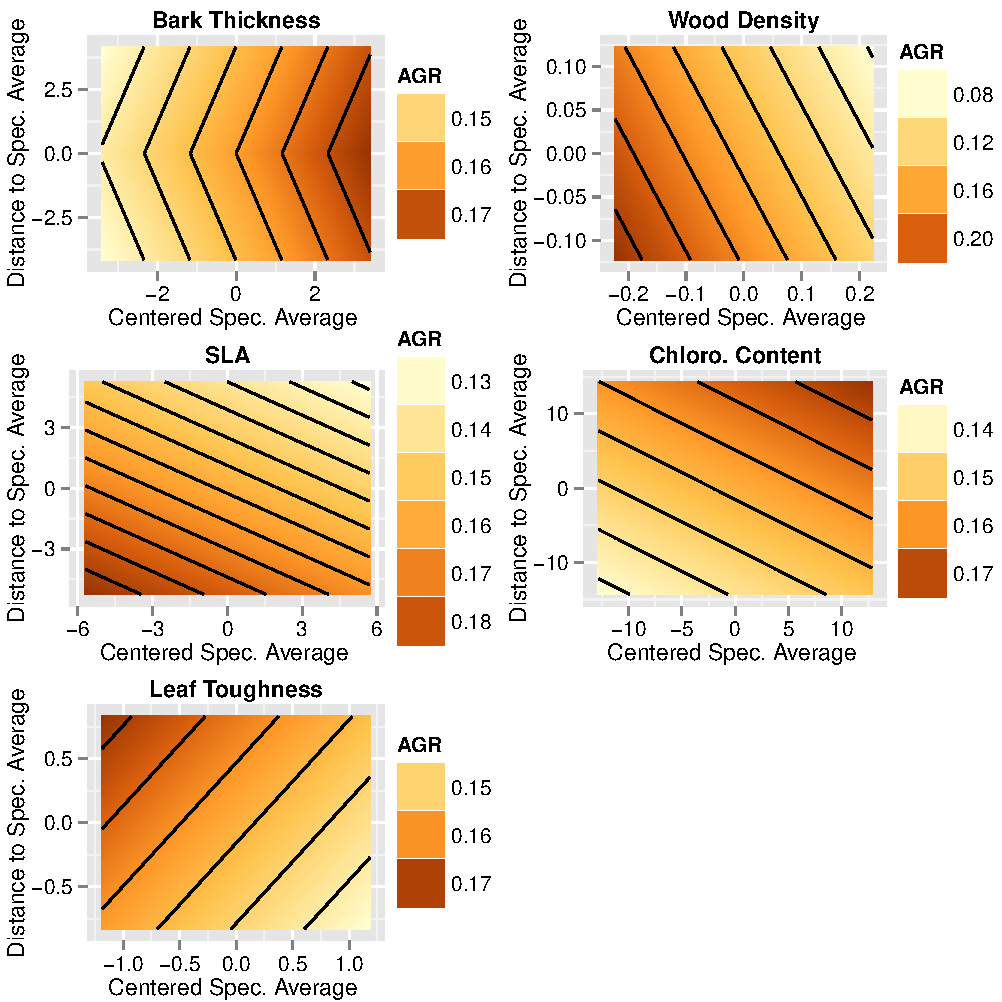
\includegraphics{figures/Sel_Traits_Simul_Pred_AGR_2015-05-22.pdf}
	\caption{\textbf{Simulations of species trait and predictions of AGR with growth models.} Surface plots of predicted AGR of simulated range of data: X-axis, centered species average trait (species average trait minus mean of all species average trait); Y-axis, individual distance to species average trait. Black lines are equal-AGR lines over the surface. For traits detail see~\autoref{tab:seltraits}.}
	\label{fig:simul}
\end{figure}